%%%%%%%%%%%%%%%%%%%%%%%%%%%%%%%%%%%%%%%%%
% Short Sectioned Assignment
% LaTeX Template
% Version 1.0 (5/5/12)
%
% This template has been downloaded from:
% http://www.LaTeXTemplates.com
%
% Original author:
% Frits Wenneker (http://www.howtotex.com)
%
% License:
% CC BY-NC-SA 3.0 (http://creativecommons.org/licenses/by-nc-sa/3.0/)
%
%%%%%%%%%%%%%%%%%%%%%%%%%%%%%%%%%%%%%%%%%

%----------------------------------------------------------------------------------------
%	PACKAGES AND OTHER DOCUMENT CONFIGURATIONS
%----------------------------------------------------------------------------------------

\documentclass[paper=a4, fontsize=11pt]{scrartcl} % A4 paper and 11pt font size

\usepackage[T1]{fontenc} % Use 8-bit encoding that has 256 glyphs
\usepackage{fourier} % Use the Adobe Utopia font for the document - comment this line to return to the LaTeX default
\usepackage[english]{babel} % English language/hyphenation
\usepackage{amsmath,amsfonts,amsthm} % Math packages

\usepackage{lipsum} % Used for inserting dummy 'Lorem ipsum' text into the template

\usepackage{sectsty} % Allows customizing section commands
\allsectionsfont{\centering \normalfont\scshape} % Make all sections centered, the default font and small caps

\usepackage{fancyhdr} % Custom headers and footers

% my packages
\usepackage{commath}
\usepackage{mathtools}
\usepackage{graphicx}
\usepackage{algorithm}
\usepackage[]{algpseudocode}
\DeclarePairedDelimiter{\ceil}{\lceil}{\rceil}
\usepackage{pgfplots}
\pgfplotsset{compat=newest}
\usepackage{hyperref}
\usepackage{enumitem}
\usepackage{subcaption}
\usepackage{multirow}
\usepackage{tkz-graph}
\usepackage{adjustbox}
\usepackage{cancel}
\usepackage[percent]{overpic}

\newlist{filedescription}{description}{2}
\setlist[filedescription]{font=\normalfont\normalcolor\bfseries\itshape}

\newlist{paramdescription}{description}{1}
\setlist[paramdescription]{font=\normalfont\normalcolor\itshape}

\pagestyle{fancyplain} % Makes all pages in the document conform to the custom headers and footers
\fancyhead{} % No page header - if you want one, create it in the same way as the footers below
\fancyfoot[L]{} % Empty left footer
\fancyfoot[C]{} % Empty center footer
\fancyfoot[R]{\thepage} % Page numbering for right footer
\renewcommand{\headrulewidth}{0pt} % Remove header underlines
\renewcommand{\footrulewidth}{0pt} % Remove footer underlines
\setlength{\headheight}{13.6pt} % Customize the height of the header

\numberwithin{equation}{section} % Number equations within sections (i.e. 1.1, 1.2, 2.1, 2.2 instead of 1, 2, 3, 4)
\numberwithin{figure}{section} % Number figures within sections (i.e. 1.1, 1.2, 2.1, 2.2 instead of 1, 2, 3, 4)
\numberwithin{table}{section} % Number tables within sections (i.e. 1.1, 1.2, 2.1, 2.2 instead of 1, 2, 3, 4)

\setlength\parindent{0pt} % Removes all indentation from paragraphs - comment this line for an assignment with lots of text

% new commands
\newcommand{\filename}[1]{\textbf{\textit{#1}}}
\newcommand{\funcname}[1]{\textbf{#1}}
\newcommand{\inv}{^{\raisebox{.2ex}{$\scriptscriptstyle-1$}}}
\renewcommand{\vec}[1]{\mathbf{#1}}

\makeatletter
\renewcommand*\env@matrix[1][*\c@MaxMatrixCols c]{%
  \hskip -\arraycolsep
  \let\@ifnextchar\new@ifnextchar
  \array{#1}}
\makeatother

\makeatletter
\def\BState{\State\hskip-\ALG@thistlm}
\makeatother

\DeclareMathAlphabet{\mathcal}{OMS}{cmsy}{m}{n}
\DeclareMathOperator*{\argmin}{arg\,min} % Jan Hlavacek

\newtheorem{theorem}{Theorem}

%----------------------------------------------------------------------------------------
%	TITLE SECTION
%----------------------------------------------------------------------------------------

\newcommand{\horrule}[1]{\rule{\linewidth}{#1}} % Create horizontal rule command with 1 argument of height

\title{	
\normalfont \normalsize 
\textsc{Mathematical foundations of computer graphics and vision} \\ [25pt] % Your university, school and/or department name(s)
\horrule{0.5pt} \\[0.4cm] % Thin top horizontal rule
\huge Exercise 5. Rigid Transform Blending and Variational Methods\\ % The assignment title
\horrule{2pt} \\[0.5cm] % Thick bottom horizontal rule
}

\author{Dongho Kang \\ \small 16-948-598} % Your name

\date{\normalsize May 21, 2017} % Today's date or a custom date

\begin{document}

\maketitle % Print the title

%----------------------------------------------------------------------------------------
%	README
%----------------------------------------------------------------------------------------

MATLAB R2016b version was used for coding and testing:

\begin{center}
MathWorks, MATLAB R2016b (9.1.0.441655) \\
64-bit (maci64) 
\end{center}

The \filename{code} directory contains the followings:

\begin{filedescription}
	\item [part2] script .m file for exercise part 2.
	\item [lotr.jpg] original image file.
	\item [results] directory contains result images of part 2.
\end{filedescription} 

For running \filename{part2.m} script, adjust options first:

\begin{paramdescription}
	\item [gf\_on] true for Gaussian filtering on. 
	\item [hd\_on] true for Heat diffusion on.
	\item [va\_on] true for variational method on.
	\item [save\_jpg] true for saving result images.
	\item [results\_dir] result images directory path.   
\end{paramdescription}

Note that \textbf{these script was only tested in MATLAB R2016b environment}.

\pagebreak

%----------------------------------------------------------------------------------------
%	PROBLEM 1
%----------------------------------------------------------------------------------------

\section{exercise part 1: Understanding and Utilizing Dual Quaternion}

%----------------------------------------------------------------------------------------
%	TASK 1
%----------------------------------------------------------------------------------------
\subsection{Task 1: Thinking about fundamental properties}

\begin{itemize}
	\item How do dual quaternions represent rotations and translations? \\

Unit dual quaternions naturally represent 3D rotation, when the dual part $\vec{q_\epsilon} = 0$ (thus $\hat{\vec{q}} = \vec{q_0} + \epsilon \vec{q_\epsilon} = \vec{q_0}$). Dual quaternion multiplication with unit dual quaternion $\hat{\vec{t}} = 1 + \frac{\epsilon}{2}(t_0 i + t_1 j + t_2 k)$ corresponds to translation by vector $(t_0, t_1, t_2)$ represent 3D translation. \cite{kavan2008geometric} \\
	
	\item What is the advantage of representing rigid transformations with dual quaternions for blending? \\
	
The linear combination of dual quaternions does not make artifacts or skin-collapsing effect, thus blending using dual quaternions is fast and more robust than using homogeneous matrix. Moreover, since dual quaternions require only 8 floats per transformation, instead of the 12 required by matrices, they are more memory efficient. \cite{kavan2008geometric}\\
	
	\item Briefly explain one fundamental disadvantage of using quaternion based shortest path blending for rotations as compared to linear blend skinning? \\
	
Dual quaternions causes "flipping artifacts" which occurs with joint rotations of more than 180 degrees. Because of its shortest path property, when the other path becomes shorter, the skin changes its shape discontinuously. \cite{kavan2008geometric}\\

\end{itemize}


%----------------------------------------------------------------------------------------
%	TASK 2 
%----------------------------------------------------------------------------------------
\subsection{Task 2: Derivations and deeper understanding}

\begin{itemize}
	\item For a dual quaternion $\hat{\vec{q}} = \text{cos} (\hat{\theta} /2) + \hat{\vec{s}} \, \text{sin} (\hat{\theta} /2)$, prove that $\hat{\vec{q}}^t = \text{cos} (t\hat{\theta} /2) + \hat{\vec{s}} \text{sin} (t\hat{\theta} /2)$ \\
	
	Starting with $\hat{\vec{q}}$:
	\begin{align}
		\hat{\vec{q}} &= \text{cos} (\hat{\theta} /2) + \hat{\vec{s}} \,\text{sin} (\hat{\theta} /2)
	\end{align}

	As $\hat{\vec{q}}^t	= \text{exp} \big(t \, \text{log}(\hat{\vec{q}}) \big)$, 
	\begin{align}
		\hat{\vec{q}}^t	&= \text{exp} \big( t \, \text{log}(\hat{\vec{q}}) \big) \\
						&= \text{exp}\Big(t \, \text{log} \big(\text{cos} (\hat{\theta} /2) + \hat{\vec{s}} \,\text{sin} (\hat{\theta} /2) \big) \Big)
	\end{align}

	Plug in $\text{log} \big(\text{cos} (\hat{\theta} /2) + \hat{\vec{s}} \,\text{sin} (\hat{\theta} /2) \big) = \hat{\vec{s}} \frac{\hat{\theta}}{2}$ to equation (1.3):
	\begin{align}
		\hat{\vec{q}}^t = \text{exp}\Big( \frac{t\hat{\theta}}{2} \,\hat{\vec{s}} \Big)
	\end{align}
	
	Let $\hat{\vec{a}} = \frac{t\hat{\theta}}{2} \,\hat{\vec{s}}$. Since $\hat{\theta} = \theta_0 + \epsilon \theta_\epsilon$ and $\hat{\vec{s}} = \vec{s}_0 + \epsilon\vec{s}_\epsilon$.
	\begin{align}
		\hat{\vec{a}} &= \frac{t\hat{\theta}}{2} \hat{\vec{s}} \\
		&= \frac{t}{2}(\theta_0 + \epsilon \theta_\epsilon)(\vec{s}_0 + \epsilon\vec{s}_\epsilon) \\
		&= \frac{t}{2} (\theta_0\vec{s}_0 + \epsilon \theta_0 \vec{s}_\epsilon + \epsilon \theta_\epsilon \vec{s}_0 + \cancelto{0}{\epsilon^2 \theta_\epsilon \vec{s}_\epsilon}) \\
		&= \underbrace{ \Big( \frac{t}{2} \theta_0\vec{s}_0 \Big) }_{\coloneqq \vec{a}_0} 
			+ \epsilon \underbrace{ \Big( \frac{t}{2} \theta_0 \vec{s}_\epsilon + \frac{t}{2} \theta_\epsilon \vec{s}_0 \Big) }_{\coloneqq \vec{a}_\epsilon }
	\end{align}
	
	Since exponential of dual quaternion is given by $e^{\hat{\vec{q}}} = \text{cos} \big( \norm{\hat{\vec{q}}} \big) + \frac{\hat{\vec{q}}}{\norm{\hat{\vec{q}}}} \text{sin} \big( \norm{\hat{\vec{q}}} \big)$, then $e^{\hat{\vec{a}}} = \text{cos} \big( \norm{\hat{\vec{a}}} \big) + \frac{\hat{\vec{a}}}{\norm{\hat{\vec{a}}}} \text{sin} \big( \norm{\hat{\vec{a}}} \big)$. Here, the norm of dual quaternion $\hat{\vec{a}}$ is $\norm{\hat{\vec{a}}} = \norm{\vec{a}_0} + \epsilon \frac{<\vec{a}_0, \vec{a}_\epsilon>}{\norm{\vec{a}_0}}$. Looking into $<\vec{a}_0, \vec{a}_\epsilon>$ and $\norm{\vec{a}_0}$,
	\begin{align}
		<\vec{a}_0, \vec{a}_\epsilon> &= <\frac{t}{2} \theta_0\vec{s}_0, \frac{t}{2} \theta_0 \vec{s}_\epsilon + \frac{t}{2} \theta_\epsilon \vec{s}_0> \\
		&= <\frac{t}{2} \theta_0\vec{s}_0, \frac{t}{2} \theta_0 \vec{s}_\epsilon> + <\frac{t}{2} \theta_0\vec{s}_0, \frac{t}{2} \theta_\epsilon \vec{s}_0> \\[0.5cm] 
		\norm{\vec{a}_0} &= \sqrt{<\vec{a}_0, \vec{a}_0>} \\
		&= \sqrt{<\frac{t}{2} \theta_0 \vec{s}_0, \frac{t}{2} \theta_0 \vec{s}_0>} 
	\end{align}
	
	Note that $<\vec{s}_0, \vec{s}_0> = 1$ and $<\vec{s}_0, \vec{s}_\epsilon> = 0$. Thus equation (1.10) and (1.12) can be expressed as follows: 
	\begin{align}
		<\vec{a}_0, \vec{a}_\epsilon> &= \Big(\frac{t}{2}\Big)^2 \theta_0 \theta_\epsilon \\[0.5cm]
		\norm{\vec{a}_0} &= \sqrt{\Big(\frac{t}{2} \theta_0 \Big)^2} = \frac{t}{2} \theta_0 
	\end{align}
	
	Plug (1.13) and (1.14) into $\norm{\hat{\vec{a}}} = \norm{\vec{a}_0} + \epsilon \frac{<\vec{a}_0, \vec{a}_\epsilon>}{\norm{\vec{a}_0}}$:
	\begin{align}
		\norm{\hat{\vec{a}}} &= \frac{t}{2} \theta_0 + \epsilon \frac{\Big(\frac{t}{2}\Big)^2 \theta_0 \theta_\epsilon}{\frac{t}{2} \theta_0}	\\
		&= \frac{t}{2} \theta_0 + \epsilon \frac{t}{2} \theta_\epsilon \\
		&= \frac{t}{2} (\theta_0 + \epsilon \theta_\epsilon) = \frac{t}{2} \hat{\theta}
	\end{align}
	
	Finally, by (1.4), (1.17) and $e^{\hat{\vec{a}}} = \text{cos} \big( \norm{\hat{\vec{a}}} \big) + \frac{\hat{\vec{a}}}{\norm{\hat{\vec{a}}}} \text{sin} \big( \norm{\hat{\vec{a}}} \big)$, 
	\begin{align}
		\hat{\vec{q}}^t &= e^{\hat{\vec{a}}} \\
		&= \text{cos} \Big( \frac{t}{2} \hat{\theta} \Big) + \frac{\hat{\vec{a}}}{\frac{t}{2}\hat{\theta}} \text{sin} \Big( \frac{t}{2} \hat{\theta} \Big) \\
		&= \text{cos} \Big( \frac{t}{2} \hat{\theta} \Big) + \frac{\cancel{\frac{t}{2} \hat{\theta}} \,\hat{\vec{s}}}{\cancel{\frac{t}{2}\hat{\theta}}} \text{sin} \Big( \frac{t}{2} \hat{\theta} \Big) \\
		&= \text{cos} \Big( \frac{t}{2} \hat{\theta} \Big) + \hat{\vec{s}} \, \text{sin} \Big( \frac{t}{2} \hat{\theta} \Big)
	\end{align}
	
	The proof has been done.
	
	\item Consider rigid transformations in the 2D $xy$-plane. For these transformations, the rotation is always around the $z$ (or $-z$)-axis, i.e. $\vec{s}_0$ is fixed to the $z$-axis. On the other hand, a dual quaternion encodes translations only along $\vec{s}_0$, which are in this case always zero, since we can only translate in the $xy$-plane. Then, how can a dual quaternion represent a rotation and translation in the $xy$-plane, such as the one depicted in Figure 1.1 (a)? 
	
	\begin{figure}[H]
	\caption{Dual quaternion (or screw) representation of 2D translation\label{fig:simple}}
	\centering
	\begin{subfigure}[b]{0.675\textwidth}
		\noindent\makebox[\textwidth]{
		  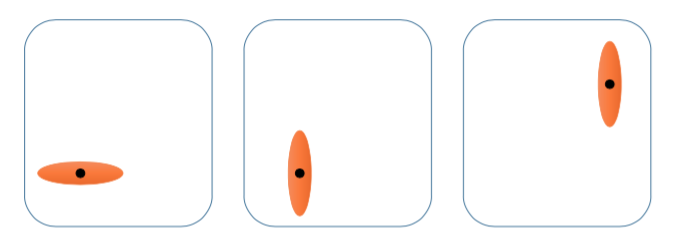
\includegraphics[width=\textwidth]{task2-fig.png}
		}
	\caption{An object (left) is first rotated around its center of mass (middle) and then translated (right)}
	\end{subfigure}
%	\hspace{0mm}
	\begin{subfigure}[b]{0.225\textwidth}
		\begin{overpic}[width=\textwidth]{task2-fig-2.png}
			\put (25,70) {$\vec{r}$}
		\end{overpic}
	\caption{Shifting the screw axis}
	\end{subfigure}
	\end{figure}
	
	For the 2D case of Figure 1.1, if the axis of dual quaternion(screw) is shifted to point $\vec{r}$ as shown in Figure 1.1 (b), such transformation can be represented as a screw axis i.e. dual quaternion. In this case, $\vec{s}_\epsilon = \vec{r} \times \vec{s}_0$. \cite{kavan2008geometric}
	
\end{itemize}

\pagebreak

%----------------------------------------------------------------------------------------
%	PROBLEM 2 
%----------------------------------------------------------------------------------------

\section{exercise part 2: Variational Methods - Denoising problems}

In this section, three different denoising methods(filtering, heat diffusion and variational approach) were implemented and compared.

\graphicspath{{results/}}
\vspace{-2mm}
\begin{figure}[H]
	\caption{Original images and noised image\label{fig:simple}}
	\centering
	\begin{subfigure}[b]{0.3\textwidth}
		\noindent\makebox[\textwidth]{
		  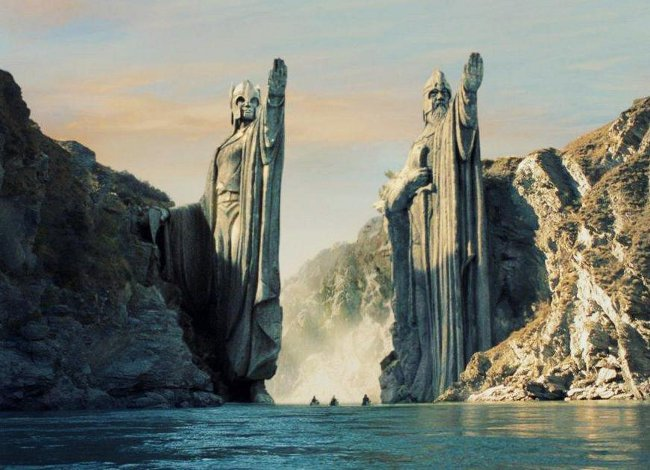
\includegraphics[width=\textwidth]{lotr.jpg}
		}
	\caption{Original image}
	\end{subfigure}
	\hspace{5mm}
	\begin{subfigure}[b]{0.3\textwidth}
		\noindent\makebox[\textwidth]{
		  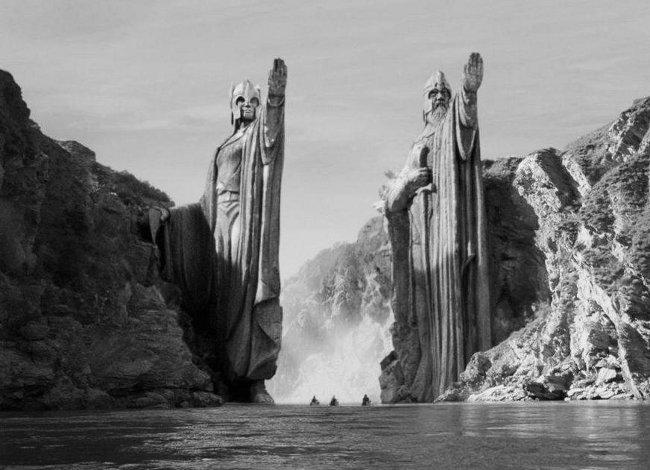
\includegraphics[width=\textwidth]{gray_image.jpg}
		}
	\caption{Grayscale image}
	\end{subfigure}
	\hspace{5mm}
	\begin{subfigure}[b]{0.3\textwidth}
		\noindent\makebox[\textwidth]{
		  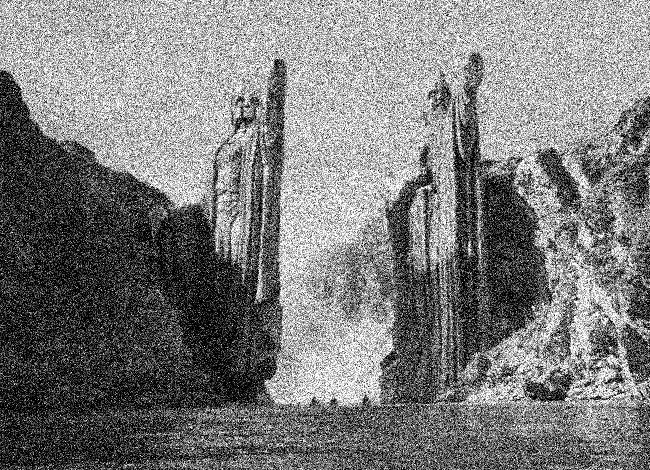
\includegraphics[width=\textwidth]{noisy_image.jpg}
		}
	\caption{Noised image}
	\end{subfigure}
\end{figure}

%----------------------------------------------------------------------------------------
%	TASK 1
%----------------------------------------------------------------------------------------

\subsection{Task 1: Filtering}

By convolution with Gaussian filter($\sigma = 0.5$), the gaussian noise was denoised. 

\vspace{-2mm}
\begin{figure}[H]
	\caption{Denoised image after filtering multiple time ($\sigma = 0.5$)\label{fig:simple}}
	\centering
	\begin{subfigure}[b]{0.45\textwidth}
		\noindent\makebox[\textwidth]{
		  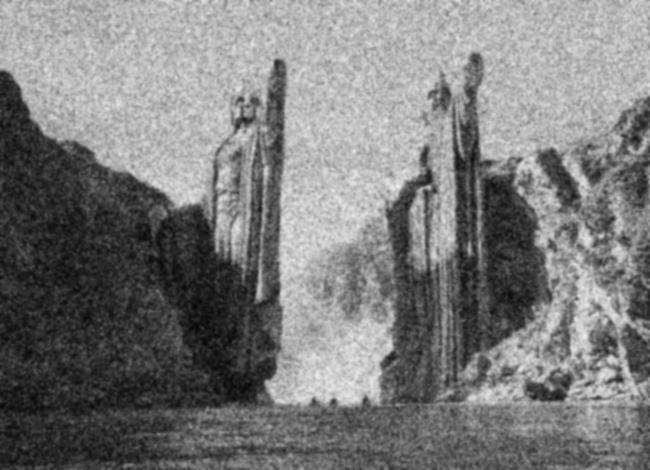
\includegraphics[width=\textwidth]{gf_8.jpg}
		}
	\caption{Filtered 8 times}
	\end{subfigure}
	\hspace{5mm}
	\vspace{5mm}
	\begin{subfigure}[b]{0.45\textwidth}
		\noindent\makebox[\textwidth]{
		  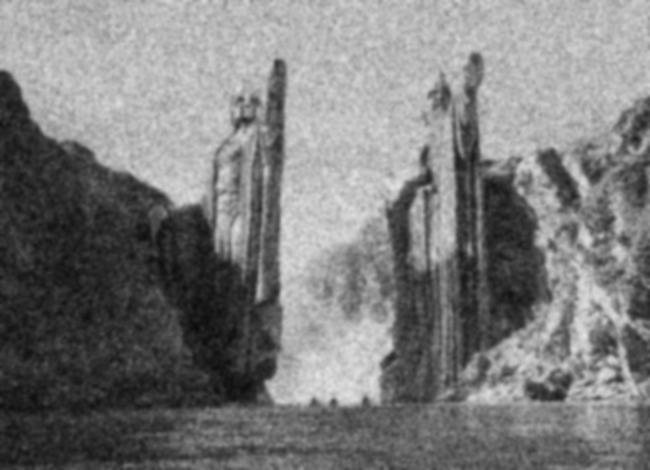
\includegraphics[width=\textwidth]{gf_16.jpg}
		}
	\caption{Filtered 16 times}
	\end{subfigure}
	\begin{subfigure}[b]{0.45\textwidth}
		\noindent\makebox[\textwidth]{
		  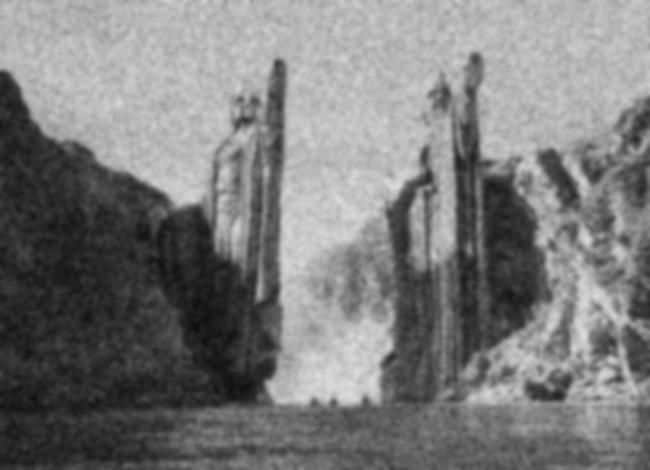
\includegraphics[width=\textwidth]{gf_24.jpg}
		}
	\caption{Filtered 24 times}
	\end{subfigure}
	\hspace{5mm}
	\begin{subfigure}[b]{0.45\textwidth}
		\noindent\makebox[\textwidth]{
		  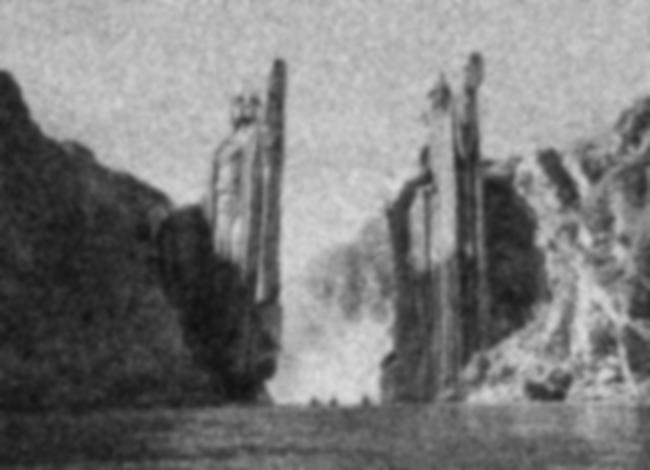
\includegraphics[width=\textwidth]{gf_32.jpg}
		}
	\caption{Filtered 32 times}
	\end{subfigure}
\end{figure}

\begin{figure}[H]
	\centering
	\noindent\makebox[0.6\textwidth]{
	  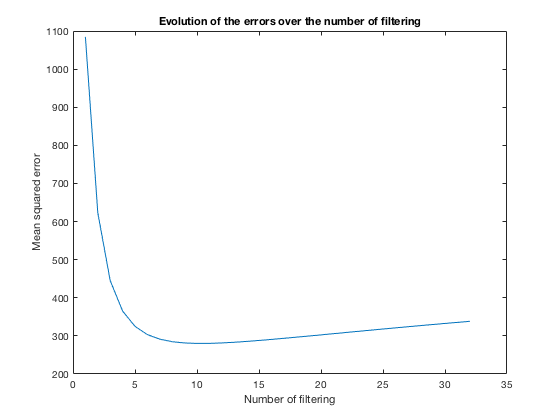
\includegraphics[width=\textwidth]{gf_errors.png}
	}
\caption{Mean square error evolution of Gaussian filtering ($\sigma = 0.5$)}
\end{figure}

As the iteration goes on, mean square error(MSE) changes as Figure 2.5. For $\sigma = 0.5$, the MSE is the smallest when the number of filtering is 10. \\ 

Results with different value of $\sigma$ are as Figure 2.6. $\sigma$ determines level of smoothing. If $\sigma$ is too small or too large, filtering does not show effective denoising.

\begin{figure}[b]
	\caption{Denoised image with different $\sigma$\label{fig:simple}}
	\centering
	\begin{subfigure}[b]{0.3\textwidth}
		\noindent\makebox[\textwidth]{
		  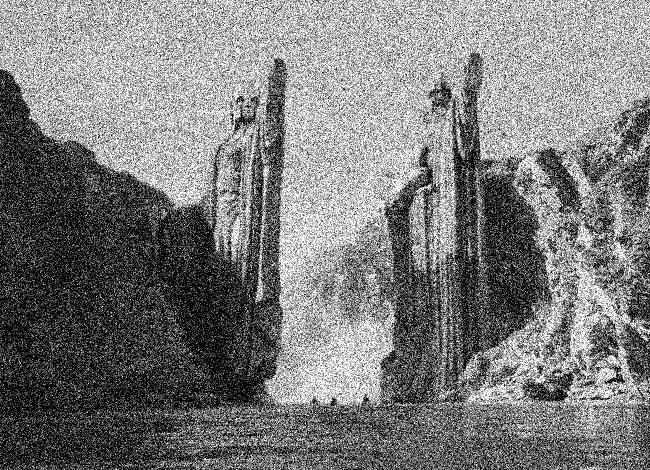
\includegraphics[width=\textwidth]{gf_32_s01.jpg}
		}
	\caption{$\sigma = 0.1$ (32 iter)}
	\end{subfigure}
	\hspace{5mm}
	\begin{subfigure}[b]{0.3\textwidth}
		\noindent\makebox[\textwidth]{
		  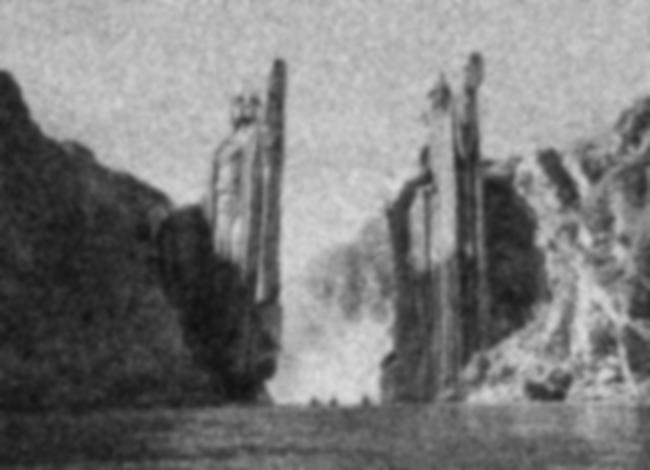
\includegraphics[width=\textwidth]{gf_32.jpg}
		}
	\caption{$\sigma = 0.5$ (32 iter)}
	\end{subfigure}
	\hspace{5mm}
	\begin{subfigure}[b]{0.3\textwidth}
		\noindent\makebox[\textwidth]{
		  
\includegraphics[width=\textwidth]{gf_32_s10.jpg}
		}
	\caption{$\sigma = 10$ (32 iter)}
	\end{subfigure}
\end{figure}


%----------------------------------------------------------------------------------------
%	TASK 2
%----------------------------------------------------------------------------------------

\subsection{Task 2: Heat diffusion}

Let $I_t$ the image at scale $t$, then heat equation is defined as follows:

\begin{equation}
	\frac{\partial I_t}{\partial t} - \Delta I_t = 0
\end{equation}

where $\Delta$ is the discrete 2D laplacian operator. For discretizing and solving (2.1), forward finite differences were used:

\begin{align}
	\frac{I_{t+1} - I_t}{\tau} &= \Delta I_t \\
	I_{t+1} &= I_t + \tau \cdot \Delta I_t
\end{align}

For 2D Laplacian at pixel $(x, y)$, the following was used:

\begin{equation}
	\Delta I(x, y) = I(x+1, y) + I(x-1, y) + I(x, y+1) + I(x, y - 1) - 4 \cdot I(x, y)
\end{equation}

Figure 2.8 shows the result images with different number of iteration of (2.3). Neumann boundary condition was used for boundary padding.

\begin{figure}[H]
	\caption{Denoised image after diffusion\label{fig:simple}}
	\centering
	\begin{subfigure}[b]{0.45\textwidth}
		\noindent\makebox[\textwidth]{
		  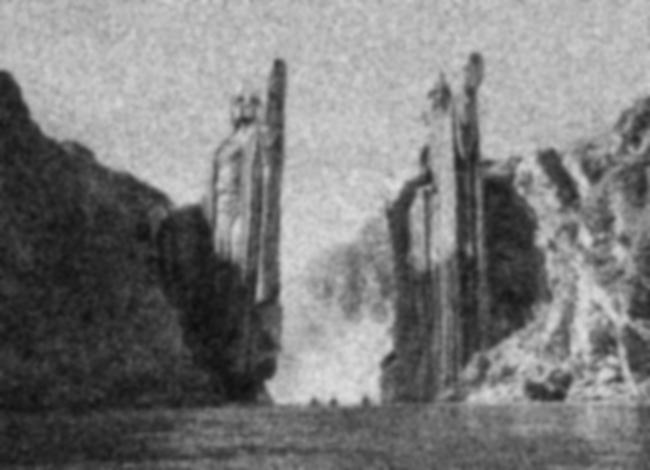
\includegraphics[width=\textwidth]{hd_25.jpg}
		}
	\caption{Diffusion at time 25}
	\end{subfigure}
	\hspace{5mm}
	\vspace{5mm}
	\begin{subfigure}[b]{0.45\textwidth}
		\noindent\makebox[\textwidth]{
		  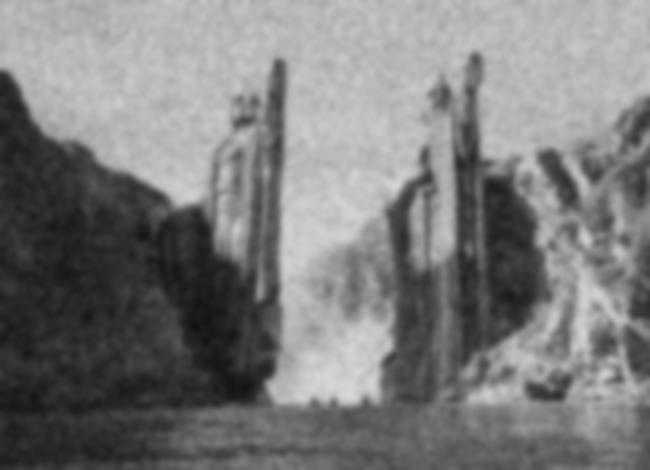
\includegraphics[width=\textwidth]{hd_50.jpg}
		}
	\caption{Diffusion at time 50}
	\end{subfigure}
	\begin{subfigure}[b]{0.45\textwidth}
		\noindent\makebox[\textwidth]{
		  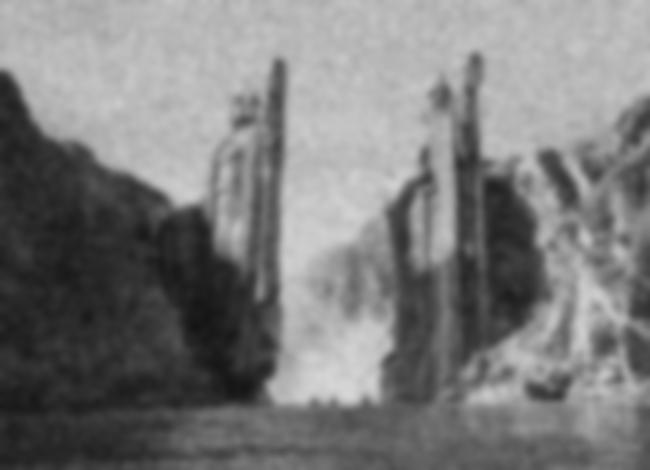
\includegraphics[width=\textwidth]{hd_75.jpg}
		}
	\caption{Diffusion at time 75}
	\end{subfigure}
	\hspace{5mm}
	\begin{subfigure}[b]{0.45\textwidth}
		\noindent\makebox[\textwidth]{
		  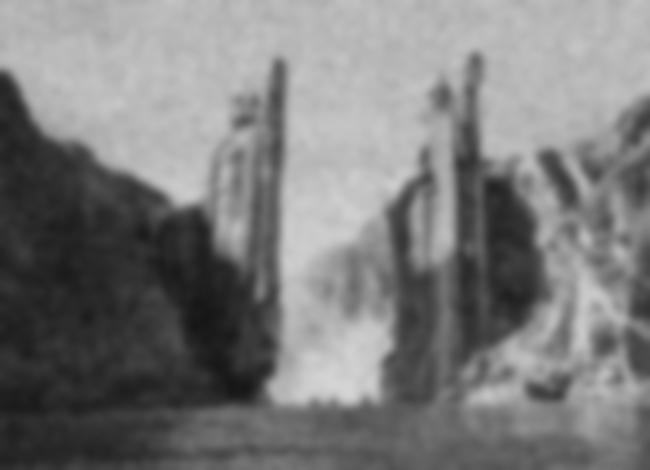
\includegraphics[width=\textwidth]{hd_100.jpg}
		}
	\caption{Diffusion at time 100}
	\end{subfigure}
\end{figure}


\begin{figure}[H]
	\centering
	\noindent\makebox[0.6\textwidth]{
	  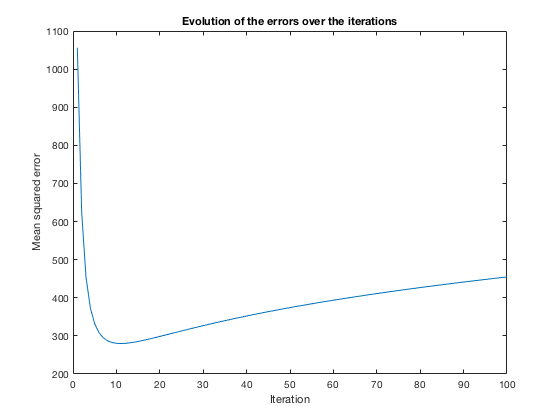
\includegraphics[width=\textwidth]{hd_errors.png}
	}
\caption{Mean square error evolution of Gaussian filtering ($\tau = 0.1$)}
\end{figure}

As the iteration goes on, mean square error(MSE) evolves as Figure 2.10. For $\tau = 0.1$, the MSE is the smallest when the number of iteration is \textbf{TODO} \\ 

Results with different value of $\tau$ are as Figure 2.11. MSE evolution is as Figure 2. (TODO) If $\tau$ is too small, it takes longer time to find a optimal solution. In contrast, if $\tau$ is too large, the MSE diverges. 

\begin{figure}[b]
	\caption{Denoised image with different $\tau$ \label{fig:simple}}
	\centering
	\begin{subfigure}[b]{0.3\textwidth}
		\noindent\makebox[\textwidth]{
		  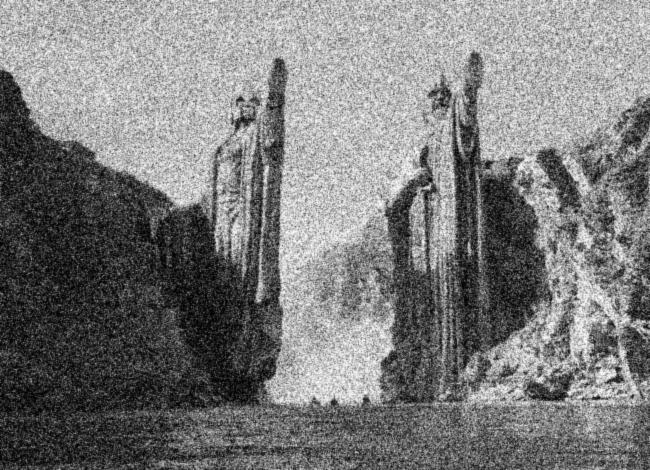
\includegraphics[width=\textwidth]{hd_25_t001.jpg}
		}
	\caption{$\tau = 0.01$ (25 iter)}
	\end{subfigure}
	\hspace{5mm}
	\begin{subfigure}[b]{0.3\textwidth}
		\noindent\makebox[\textwidth]{
		  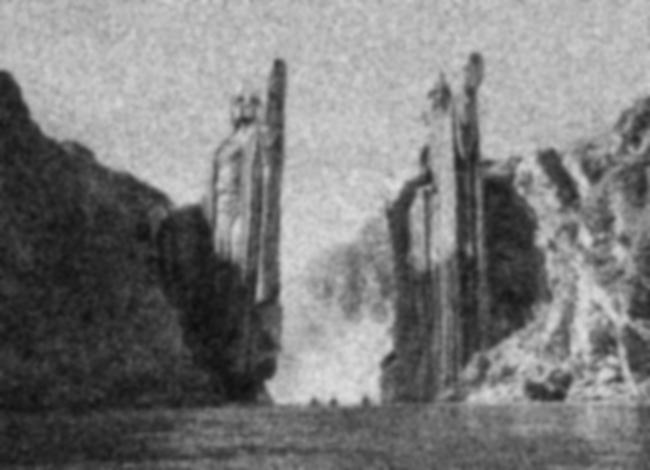
\includegraphics[width=\textwidth]{hd_25.jpg}
		}
	\caption{$\tau = 0.1$ (25 iter)}
	\end{subfigure}
	\hspace{5mm}
	\begin{subfigure}[b]{0.3\textwidth}
		\noindent\makebox[\textwidth]{
		  
\includegraphics[width=\textwidth]{hd_25_t05.jpg}
		}
	\caption{$\tau = 0.5$ (25 iter)}
	\end{subfigure}
\end{figure}

\begin{figure}[H]
	\caption{Denoised image with different $\tau$ \label{fig:simple}}
	\centering
	\begin{subfigure}[b]{0.45\textwidth}
		\noindent\makebox[\textwidth]{
		  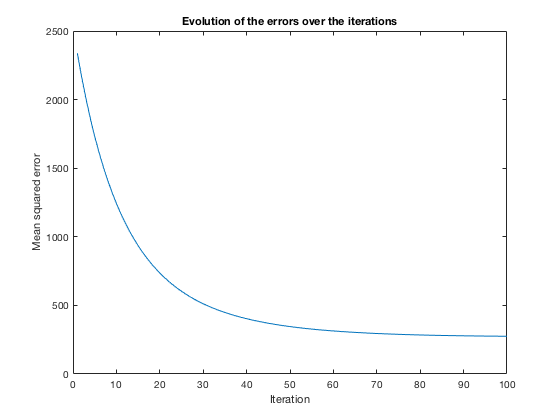
\includegraphics[width=\textwidth]{hd_errors_t001.png}
		}
	\caption{$\tau = 0.01$}
	\end{subfigure}
	\begin{subfigure}[b]{0.45\textwidth}
		\noindent\makebox[\textwidth]{
		  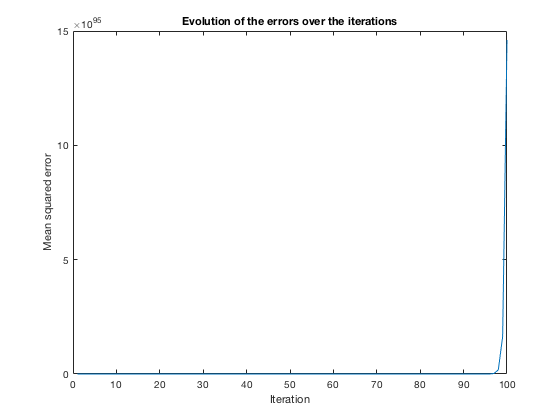
\includegraphics[width=\textwidth]{hd_errors_t05.png}
		}
	\caption{$\tau = 0.5$ (diverged)}
	\end{subfigure}
\end{figure}


%----------------------------------------------------------------------------------------
%	TASK 3
%----------------------------------------------------------------------------------------

\subsection{Task 3: Variational approach}

%----------------------------------------------------------------------------------------
\subsubsection{Description}

Finally, variational approach was implemented. This method considers the image as function of the space of all images. 
TODO

\paragraph{Derivation of Euler-Lagrange equation}

The energy function for denoising problem can be defined as follows:
\begin{align}
	E(I) = \int_{\Omega}\Big[\big(I(\vec{x}) - I_0(\vec{x})\big)^2 + \lambda \norm{\nabla_{\vec{x}} I(\vec{x})}^2 \Big]	d\vec{x}
\end{align}

where, $\Omega = \mathbb{R}^2$ is the domain of the 2D image, $I_0$ the noisy image, and $\lambda$ a regularization parameter. $I, I_0 \in \mathcal{V} = \mathcal{L}^2(\Omega)$. \\

Let's define the function $L(I, \nabla_{\vec{x}} I, \vec{x})$ as follows: 
\begin{align}
	L(I, \nabla_{\vec{x}} I, \vec{x}) = \Big[\big(I(\vec{x}) - I_0(\vec{x})\big)^2 + \lambda \norm{\nabla_{\vec{x}} I(\vec{x})}^2 \Big]
\end{align}

Then the G\^ateaux derivative is given by 
\begin{align}
	\delta E(I;h) &= \lim_{\alpha \to 0} \frac{1}{\alpha}\Big(E(I + \alpha h) - E(I)\Big) \\
	&= \lim_{\alpha \to 0} \frac{1}{\alpha} \int_\Omega \Big(L(I + \alpha h, \nabla_{\vec{x}} I + \alpha \nabla_{\vec{x}} h, \vec{x}) - L(I, \nabla_{\vec{x}} I, \vec{x}) \Big) d\vec{x} \\ 
	\shortintertext{apply matrix Taylor expansion:} 
	&= \lim_{\alpha \to 0} \frac{1}{\alpha} \int_\Omega \Big( \cancel{L(I, \nabla_{\vec{x}} I, \vec{x})} + \alpha h \cdot \frac{\partial L}{\partial I} + \alpha \nabla_{\vec{x}} h \bullet \frac{\partial L}{\partial (\nabla_{\vec{x}} I)} + o(\alpha^2) - \cancel{L(I, \nabla_{\vec{x}} I, \vec{x})} \Big) d\vec{x} \\
	&= \int_\Omega \Big( h \cdot \frac{\partial L}{\partial I} + \nabla_{\vec{x}} h \bullet \frac{\partial L}{\partial (\nabla_{\vec{x}} I)} \Big) d\vec{x} \\
	\shortintertext{apply integration by parts and $h = 0$ on boundary :} 
	&= \int_\Omega h \cdot \frac{\partial L}{\partial I} \, d\vec{x} + \cancelto{0}{h \cdot \frac{\partial L}{\partial (\nabla_{\vec{x}} I)} \Bigg|_\Omega}  - \int_\Omega h \cdot \nabla_{\vec{x}} \bullet \frac{\partial L}{\partial (\nabla_{\vec{x}} I)} \, d\vec{x} \\
	&= \int_\Omega h(\vec{x}) \cdot \Big( \frac{\partial L}{\partial I} - \nabla_{\vec{x}} \bullet \frac{\partial L}{\partial (\nabla_{\vec{x}} I)} \Big) \, d\vec{x}
\end{align} \\

Remark following theorem:

\begin{theorem}
	If $\hat{u}$ is an extremum of a functional $E : \mathcal{V} \rightarrow \mathbb{R}$, then \\
	\begin{equation*}
		\delta E(\hat{u}, h) = 0 \quad \forall h \in \mathcal{V}.
	\end{equation*} \\
\end{theorem}

By (2.8) and \textbf{Theorem 1}, 
\begin{equation}
	\frac{\partial L}{\partial I} - \nabla_{\vec{x}} \bullet \frac{\partial L}{\partial (\nabla_{\vec{x}} I)} = 0	
\end{equation}


Plug (2.2) into (2.9): 
\begin{align}
	\frac{\partial L}{\partial I} &= 2 \big(I - I_0) \\
	\nabla_{\vec{x}} \bullet \frac{\partial L}{\partial (\nabla_{\vec{x}} I)} &= 2 \lambda \, \nabla_{\vec{x}} \bullet (\nabla_{\vec{x}} I) \\ 
	&= 2 \lambda \, \textbf{div}(\nabla_{\vec{x}} I)
\end{align}

\paragraph{Vectorization and Linear operation}



%----------------------------------------------------------------------------------------
\subsubsection{Results}

\begin{figure}[H]
	\caption{Denoised image with variational method\label{fig:simple}}
	\centering
	\begin{subfigure}[b]{0.45\textwidth}
		\noindent\makebox[\textwidth]{
		  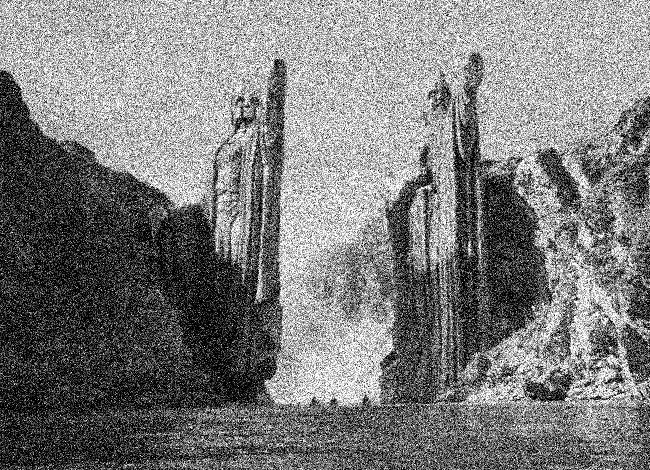
\includegraphics[width=\textwidth]{noisy_image.jpg}
		}
	\caption{Noisy image}
	\end{subfigure}
	\hspace{5mm}
	\vspace{5mm}
	\begin{subfigure}[b]{0.45\textwidth}
		\noindent\makebox[\textwidth]{
		  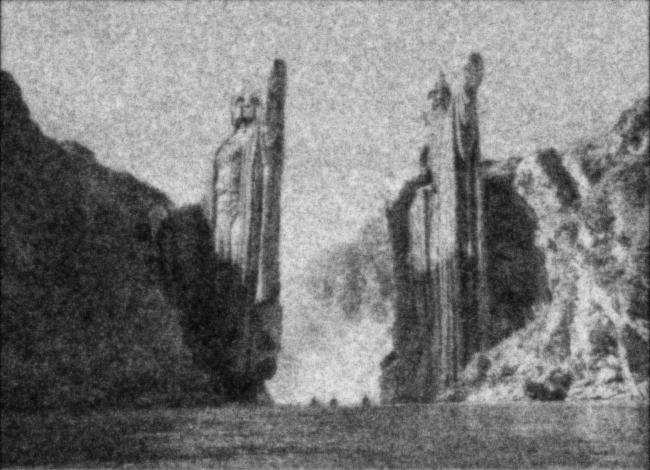
\includegraphics[width=\textwidth]{va.jpg}
		}
	\caption{Variational denoising}
	\end{subfigure}
\end{figure}



\begin{figure}[H]
	\caption{Denoised image with different $\tau$\label{fig:simple}}
	\centering
	\begin{subfigure}[b]{0.3\textwidth}
		\noindent\makebox[\textwidth]{
		  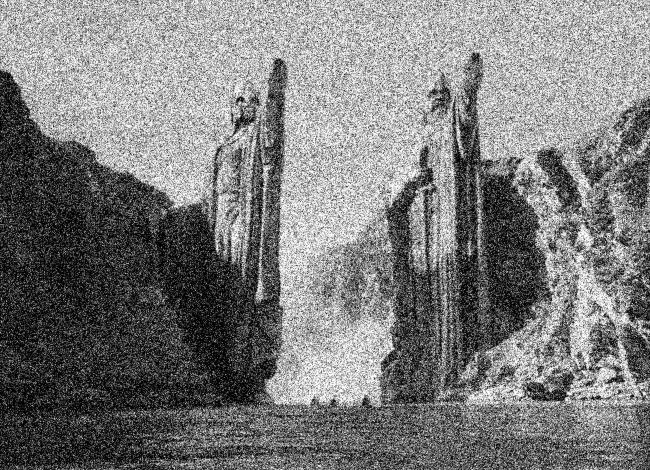
\includegraphics[width=\textwidth]{va_l01.jpg}
		}
	\caption{$\lambda = 0.1$ (MSE $= 530.9$)}
	\end{subfigure}
	\hspace{5mm}
	\begin{subfigure}[b]{0.3\textwidth}
		\noindent\makebox[\textwidth]{
		  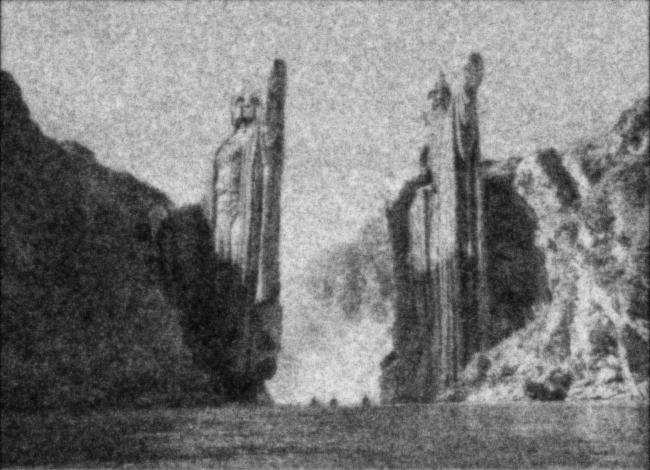
\includegraphics[width=\textwidth]{va.jpg}
		}
	\caption{$\lambda = 2$ (MSE $= 311.5$)}
	\end{subfigure}
	\hspace{5mm}
	\begin{subfigure}[b]{0.3\textwidth}
		\noindent\makebox[\textwidth]{
		  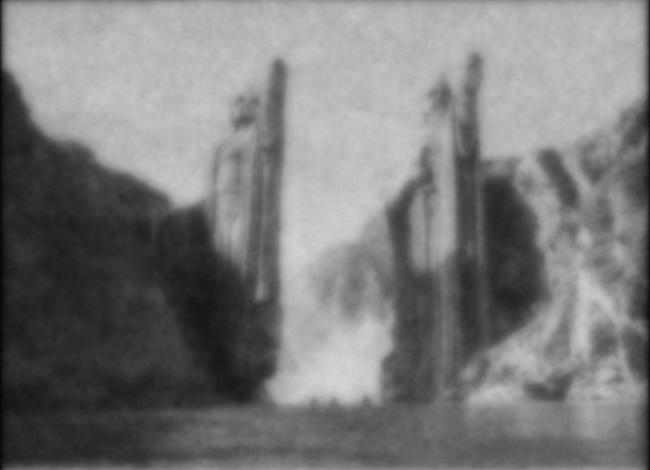
\includegraphics[width=\textwidth]{va_l20.jpg}
		}
	\caption{$\lambda = 20$ (MSE $= 1416.4$)}
	\end{subfigure}
\end{figure}





%----------------------------------------------------------------------------------------
%	TASK 4
%----------------------------------------------------------------------------------------

\subsection{Task 4: Comparison}

\begin{itemize}
	\item How can you describe the results? Does any of these methods give better results than the others? 
	\item What are the benefits and drawbacks of each methods?
	\item Can you explain the motivations behind each of the methods? 
\end{itemize}


%----------------------------------------------------------------------------------------
%	REFERENCES
%----------------------------------------------------------------------------------------

\bibliography{reference} 
\bibliographystyle{ieeetr}

\end{document}
